\section{Architektur}
\label{sec:architecture}

Die Architektur des Prototypen wurde bewusst simpel gehalten und ist
in~\autoref{fig:prototype_architecture} ersichtlich.

\begin{figure}[H]
    \centering
    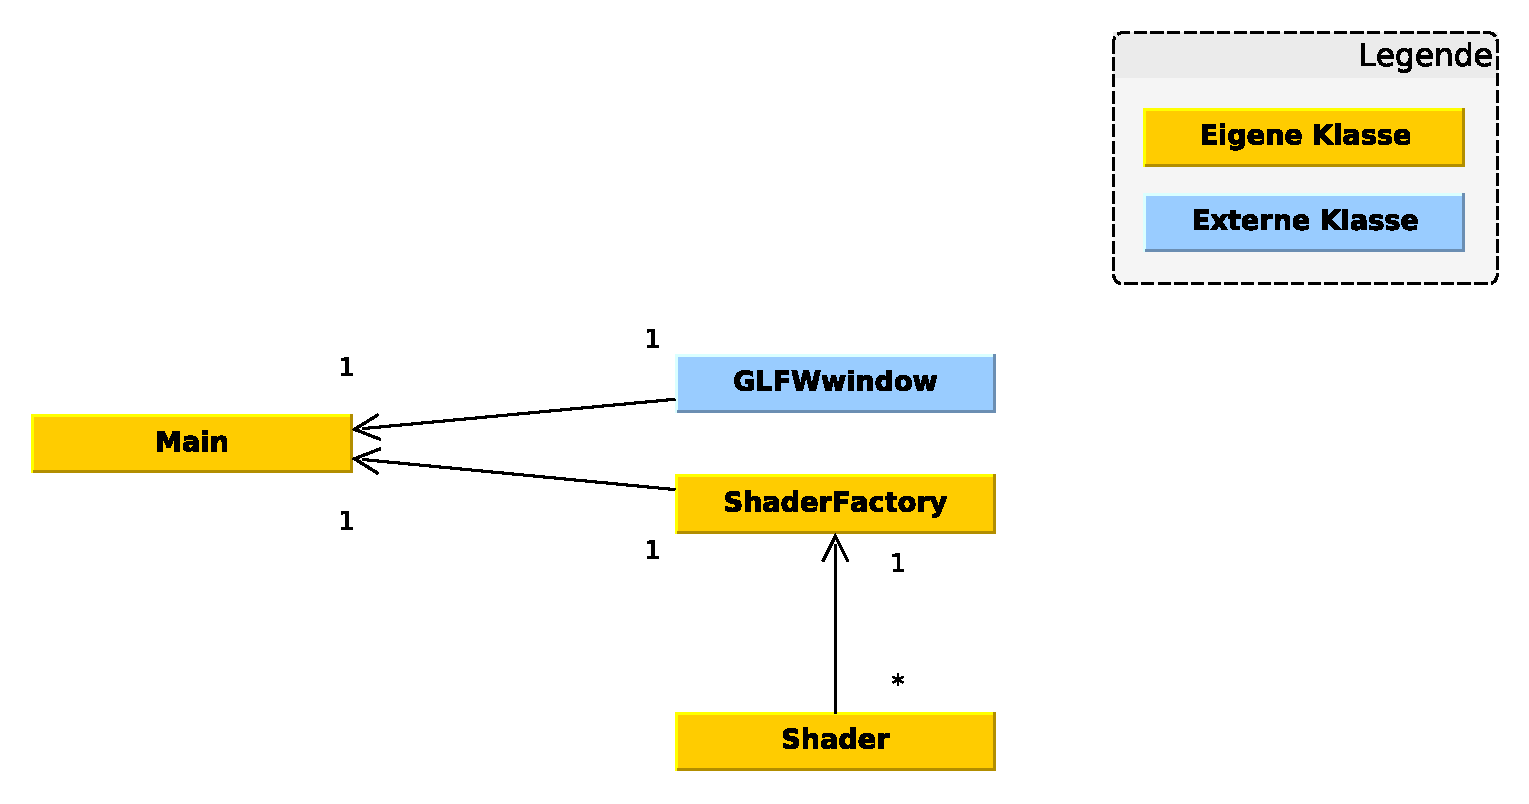
\includegraphics[width=0.8\textwidth]{img/prototype_class_diagram.pdf}
    \caption{Architektur des Prototypen\protect\footnotemark}\label{fig:prototype_architecture}
\end{figure}
\footnotetext{Eigene Darstellung mittels yEd.}

\subsection{Programmablauf}
\label{subsec:program_sequence}

Wie in~\autoref{fig:prototype_architecture} ersichtlich ist, besteht die
Applikation hauptsächlich aus der Hautpklasse \textit{main}. Diese
initialisiert mittels GLEW OpenGL und erstellt mittels GLFW ein Fenster sowie
einen OpenGL-Kontext. Danach wird eine Instanz der Klasse
\textit{ShaderFactory} erstellt, welche ihrerseits alle verfügbaren GLSL-Shader
in einem gegebenen Verzeichnis lädt. Bei diesem Prototypen kommt jedoch nur ein
Shader zum Einsatz --- bestehend aus einem Vertex- sowie einem Fragment-Teil.

Die Applikation läuft danach in einer Endlosschleife, hört dabei aber
auf Events in Form von Keyboard-Eingaben. So kann die Applikation
jederzeit mit der Abbruch-Taste (ESC, Escape) beendet werden.

Die hauptsächliche Idee der Applikation ist die, dass diese im Rendering-Teil einen
Vertex- sowie einen Fragment-Shader lädt und ausführt. Dazu wird via OpenGL ein
Rechteck über die verfügbare Fläche des Fensters ausgegeben.  Der Vertex-Shader
adressiert schliesslich das von OpenGL gezeichnete Rechteck.  Das eigentliche
Rendering von impliziten Oberflächen geschieht dann im Fragment-Shader. Dies
ist in der untenstehenden Abbildung~\ref{fig:prototype_shaders} verdeutlicht.

\begin{figure}[H]
    \centering
    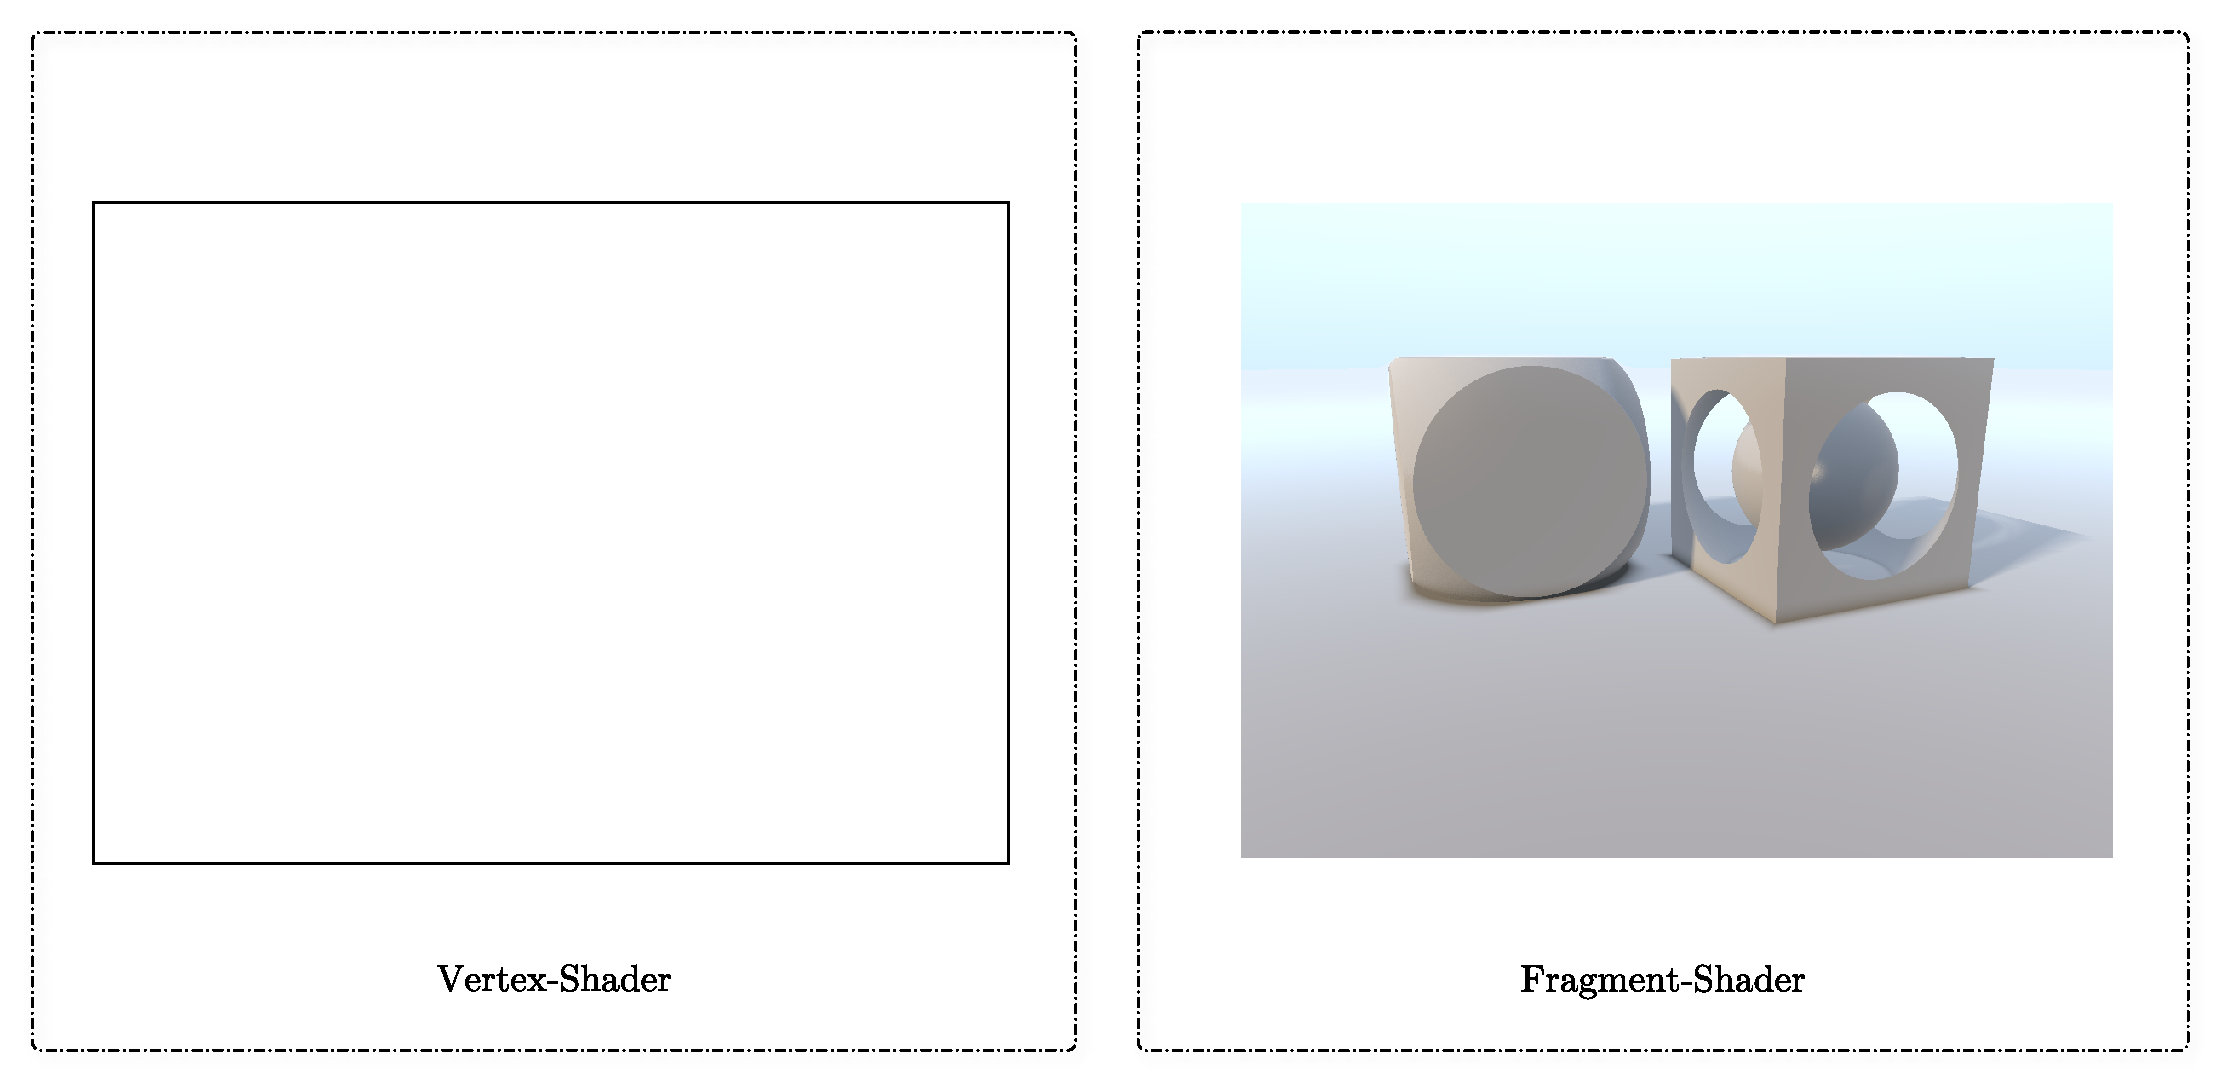
\includegraphics[width=0.8\textwidth]{img/prototype_shaders.pdf}
    \caption{Bildliche Darstellung der Funktionsweise von Vertex- und
        Fragment-Shader der Applikation\protect\footnotemark}\label{fig:prototype_shaders}
\end{figure}
\footnotetext{Eigene Darstellung mittels yEd.}
